% --- Chapter appendices, numbered <chapter>.A, .B, ... -----------------------
\renewcommand{\thesection}{\thechapter.\Alph{section}}
\setcounter{section}{0}

\section{Survival of small populations}
\label{m:app:smallpops}

\Cref{m:sec:gw} defined the binary Galton--Watson process from a single
progenitor, and \ChA{} follows that process through: whether it dies out, how
long it takes, and what remains of it when the survivors are gathered together.
One question belongs here rather than there, because it concerns founding cohorts
rather than late-time behaviour and is used by the modelling chapters that follow.
How long does a small population last, and how much difference does the size of
the founding group make?

Near criticality, with $p$ and $1-p$ each close to a half, a lineage dies at its
first round almost half the time. Should it survive one generation, both its
offspring fail at their own first attempt with probability around $0.25$, so the
lineage reaches the second generation only with probability about $0.375$:
\begin{equation*}
0.375\approx
\underbrace{(1-0.5)}_{\text{no extinction at the first step}}\times
\underbrace{(1-0.5\times0.5)}_{\text{nor at the second}} .
\end{equation*}
More generally, survival to a given generation is obtained by iterating
\cref{m:eq:SnIter}. At exactly critical branching the extinction probabilities for
$n=1,2,3,4$ are $u_n = 0.500,\ 0.625,\ 0.695,\ 0.741$ to three significant figures,
so the probability of survival decays quickly over the first few rounds, and does
so almost as fast just above criticality as just below (\cref{m:fig:earlySn}).

\begin{figure}[ht]
\centering
  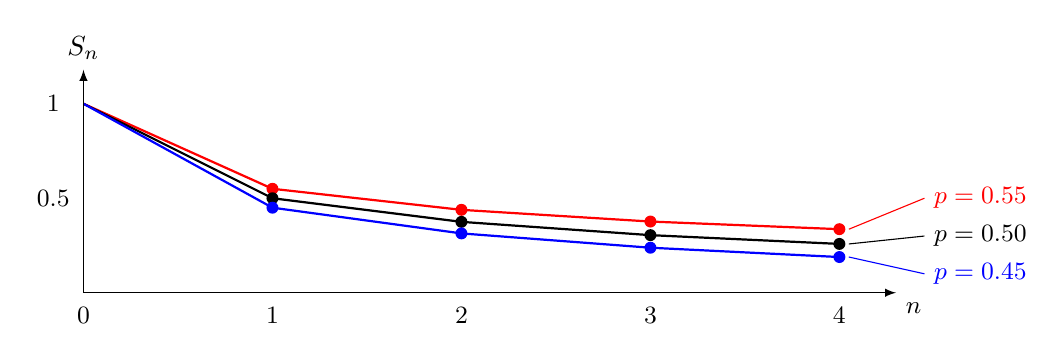
\begin{tikzpicture}[scale = 2.4]
    \foreach \x/\y/\color in {1/0.55/red, 2/0.4386250/red, 3/0.3766719/red, 4/0.336304/red,
                              1/0.5/black, 2/0.375/black, 3/0.3046875/black, 4/0.25827/black,
                              1/0.449999/blue, 2/0.313874/blue, 3/0.2381546/blue, 4/0.188816/blue}
      \fill[color=\color] (\x, \y) circle (0.9pt);
    \draw[red, thick] (0, 1) -- (1, 0.55) -- (2, 0.4386250) -- (3,0.3766719) -- (4,0.336304);
    \draw[black, thick] (0, 1)--(1,0.5) --  (2,0.375) -- (3,0.304687) -- (4,0.25827);
    \draw[blue, thick] (0, 1)--(1,0.449999)  --  (2,0.313874) -- (3,0.238154) -- (4,0.18881);
    \draw[-latex] (0,0) -- (4.3,0) node[below right, font=\small] {$n$};
    \draw[-latex] (0,0) -- (0,1.18) node[above] {$S_n$};
    \foreach \x/\lab in {0/0, 1/1, 2/2, 3/3, 4/4} \node[font=\small] at (\x, -0.12) {\lab};
    \foreach \y/\lab in {0.5/0.5, 1/1} \node[font=\small] at (-0.16, \y) {\lab};
    \draw[red,  thin] (4.05,0.336) -- (4.45,0.50);
    \draw[black,thin] (4.05,0.258) -- (4.45,0.30);
    \draw[blue, thin] (4.05,0.189) -- (4.45,0.10);
    \node[red,  font=\small, anchor=west] at (4.45, 0.50) {$p=0.55$};
    \node[black,font=\small, anchor=west] at (4.45, 0.30) {$p=0.50$};
    \node[blue, font=\small, anchor=west] at (4.45, 0.10) {$p=0.45$};
  \end{tikzpicture}
\caption{Survival probability over the first four generations from a single
progenitor. Even in the supercritical case ($p=0.55$) the early decay is steep, and
the three curves have barely separated by $n=4$.}
\label{m:fig:earlySn}
\end{figure}

\subsubsection*{An initial cohort of size \texorpdfstring{$k$}{k}}

Suppose now $Z_0=k$: the process begins with a group rather than an individual.
Under supercritical branching, growth becomes more predictably exponential as the
count rises, because a large number of individuals lets the expected dynamics show
through the noise. The founding cohort is precisely the regime in which that noise
dominates instead.

The lineages are independent and each is extinct by generation $n$ with probability
$u_n$, so all $k$ have gone with probability $u_n^{\,k}$ and
\begin{equation}
\label{m:eq:Snk}
S^{(k)}_n = 1-u_n^{\,k} .
\end{equation}
Letting $n\to\infty$, the survival probability of a single lineage tends to the
attracting fixed point of \cref{m:eq:SnIter}, which is $0$ for $p\le\tfrac12$ and
$(2p-1)/p$ for $p>\tfrac12$; both are established in \ChA. A single lineage is
therefore ultimately extinct with certainty below criticality and with probability
$(1-p)/p$ above it, so that the establishment probability of the whole cohort is
$0$ for $p\le\tfrac12$ and $1-\bigl((1-p)/p\bigr)^k$ for $p>\tfrac12$: a larger
cohort helps decisively above criticality and, in the long run, not at all below
it. \Cref{m:fig:kvals,m:fig:kvals2} show $S^{(k)}_n$ through
$500$ generations for $k=1,10,100,1000$. The improvement in longevity that a larger
first cohort buys is acutely sensitive to criticality, and the two panels of
\cref{m:fig:kvals2} differ only in the third decimal place of $p$.

\begin{figure}[ht]
\centering

\includegraphics[width=0.52\textwidth]{kvals.png}
\caption{Survival probability $S^{(k)}_n$ from \cref{m:eq:Snk} out to $500$
generations at exact criticality, $p=0.5$, for $k=1,10,100,1000$ (blue through to
red). A larger founding cohort buys longevity, but at criticality every curve is
still headed for zero.}
\label{m:fig:kvals}
\end{figure}

\begin{figure}[ht]
\centering

\includegraphics[width=0.44\textwidth]{kvals505.png}
\hfill

\includegraphics[width=0.44\textwidth]{kvals495.png}
\caption{As \cref{m:fig:kvals}, but with $p$ displaced slightly from criticality:
$p=0.505$ on the left (supercritical), $p=0.495$ on the right (subcritical). A
displacement of half a per cent separates curves that were nearly coincident in
\cref{m:fig:kvals}.}
\label{m:fig:kvals2}
\end{figure}
